\begin{figure*}[t]
\centering
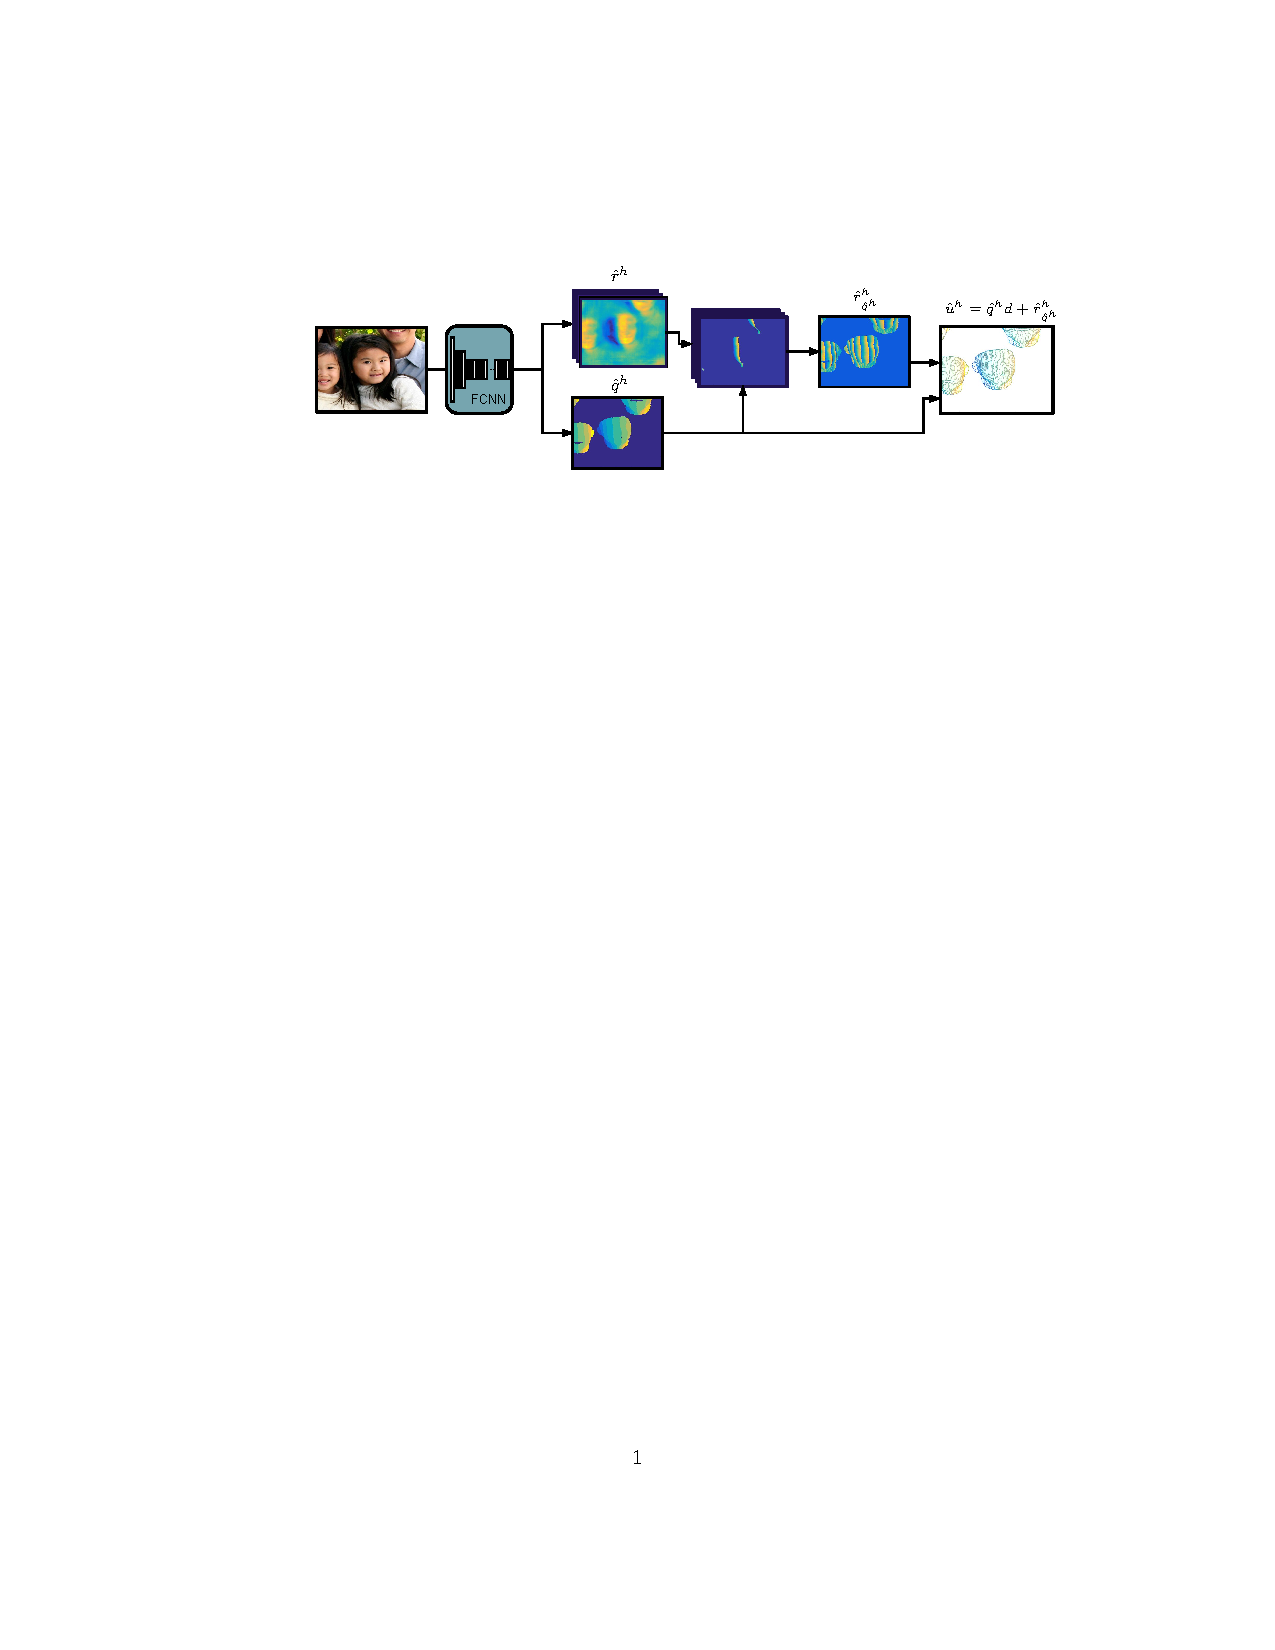
\includegraphics[trim={5.2cm 20cm 3.7cm 4.5cm}, clip, width=0.95\linewidth ]{Figures/Flow}
\caption{Proposed Quantized Regression Approach for the horizontal correspondence signal: The continuous  signal is regressed by first estimating a grossly quantized (or, discretized) function  through a classification branch. For each quantized value $\hat{q}^h$ we use a separate residual regression unit's prediction, $\hat{r}^h_{\hat{q}^h}$, effectively multiplexing the different residual predictions. These are added to the quantized prediction, yielding a smooth and accurate correspondence field. }
\vspace{-0.35cm}
\label{fig:Pipeline}
\end{figure*}


Having described how we establish our supervision signal, we now turn to the task of estimating it through a convolutional neural network (CNN). 
Our aim is to estimate at any image pixel that belongs to a face region the values of  $\bm{u} =[u^h, u^v]$. We need to also identify non-face pixels,  e.g. by predicting a `dummy' output. 

One can phrase this problem as a generic regression task and attack it with the powerful machinery of CNNs. Unfortunately, the best performance that we could obtain this way was quite underwhelming, apparently due to the task's complexity. Our approach is to quantize and estimate the quantization error separately for each quantized value. Instead of directly regressing $u$, the quantized regression approach lets us solve a set of easier sub-problems, yielding improved regression results.

In particular,	instead of  using a CNN as a `black box' regressor, we draw inspiration from the success of recent works on semantic part  segmentation \citep{tsogkas2015deep,CP2016Deeplab}, and landmark classification \citep{bulat2016human,bulat2016two}. These works have shown that CNNs can deliver remarkably accurate predictions when trained to predict \textit{categorical variables}, indicating for instance the facial part or landmark corresponding to each pixel. 
	
Building on these successes, we propose a hybrid method that combines a classification with a regression problem. Intuitively, we first identify a coarser face region that can contain each pixel, and then obtain a refined, region-specific prediction of the pixel's $U-V$  field. As we will describe below, this yields substantial gains in performance when compared to the baseline of a generic regression system. 

For the human bodies, the regions are modeled by hand and for the facial regions, we use a simple geometric approach:
We tesselate the template's surface with a cartesian grid, by uniformly and separately quantizing the $u^h$ and $u^v$ coordinates into $K$ bins, where $K$ is a design parameter. For any image that is brought into correspondence with the template domain, this induces a discrete labelling, which can be recovered by training a  CNN for classification.
	
\begin{figure}[h]
\begin{center}
   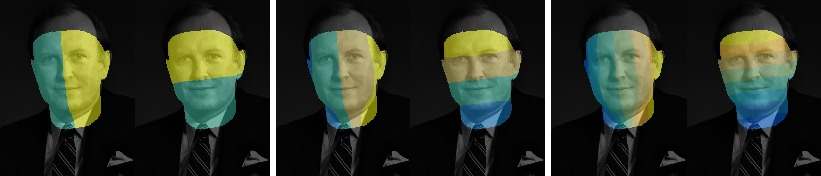
\includegraphics[width=1\linewidth ]{Figures/discreteFaces}
\end{center}
   \caption{Horizontal and vertical tesselations obtained using $K=2,4$ and $8$ bins.}
   \vspace{-0.5cm}
\label{fig:DiscreteFaces}
\end{figure}

On Fig.~\ref{fig:DiscreteFaces}, the tesselations of different granularities are visualized. For a sufficiently large value of $K$ even a plain classification result could provide a reasonable estimate of the pixel's correspondence field, albeit with some staircasing effects. The challenge here is that as the granularity of these discrete labels becomes increasingly large, the amount of available training data decreases and label complexity increases. A more detailed analysis on the effect of label-space granularity to segmentation performance is provided in supplementary materials.

We propose to combine powerful classification results with a regression problem that will yield a  refined  correspondence estimate. For this, we compute the residual between the desired and quantized $U-V$  coordinates and add a separate module that tries to regress it. We train a separate regressor per facial region, and at any pixel only penalize the regressor loss for the responsible face region. We can interpret this form as a `hard' version of a mixture of regression experts \citep{JordanJ94}. 

The horizontal and vertical components $u^h,u^v$ of the correspondence field are predicted separately. This results in a substantial reduction in computational and sample complexity -  For $K$ distinct U and V bins we have $K^2$ regions; the classification is obtained by combining 2 $K$-way classifiers. Similarily, the regression mapping involves $K^2$ regions, but only uses $2 K$ one-dimensional regression units. The pipeline for quantized face shape regression is provided in Fig.~\ref{fig:Pipeline}.

We now detail the training and testing of this network;  for simplicity we only describe the horizontal component of the mapping. 
From the ground truth construction, every position $\bm{x}$ is associated with a scalar ground-truth value $u^h$. Rather than trying to predict $u^h$ as is, we transform it into a pair of discrete $q^h$ and continuous $r^h$ values, encoding the quantization and residual respectively:
\begin{equation} 
q^h =  \lfloor {\frac{u^h}{d}} \rfloor, \quad  r_i^h =   \left(u^h_i - q^h_i d  \right),
\end{equation}
where $d = \frac{1}{K}$ is the quantization step size (we consider $u^h,u^v$ coordinates to lie in $[0,1$]).

Given a common CNN trunk, we use two classification branches to predict $q^h, q^v$ and two regression branches to predict $r^h,r^v$ as convolution layers with kernel size $1\times1$. As mentioned earlier, we employ separate regression functions per region, which means that at any position we have $K$ estimates of the horizontal residual vector, $\hat{r}^h_{i},~i=1,\ldots,K$.

At test time, we let the network predict the discrete bin $\hat{q}^h$ associated with every input position, and then use the respective regressor output $\hat{r}^h_{\hat{q}^h}$ to obtain an estimate of $u$:
\begin{equation}   
\hat{u}^h =  \hat{q}^h d + \hat{r}^h_{\hat{q}^h}
\end{equation}

For the $q^h$ and $q^v$, which are modeled as categorical distributions,  we use  softmax followed by the cross entropy loss. For estimating $\hat{r}^h$ and $\hat{r}^v$, we use a normalized version of the smooth $L_1$ loss~\citep{girshick2015fast}. The normalization is obtained by dividing the loss by the number of pixels that contribute to the loss.


\subsection{Quantized Regression as Mixture of Experts}
\label{sec:MOE}

In our formulation,  $\hat{q}^h$ is modeled using a categorical distribution and is trained using softmax followed by cross entropy loss. This reconstruction can also be seen as:
\begin{equation}
\hat{u}^h = \sum_{i=0}^{K-1}  1_{(\hat{q}^h=i)}  (  i \cdot d + \hat{r}^h_{i}),
\end{equation}
where $(  i \cdot d + \hat{r}^h_{i})$ is the reconstruction by the $i_{\mathrm{th}}$ regressor and $1_{(\hat{q}^h=i)}$ is an indicator function, determining when the $i_{\mathrm{th}}$ regressor is active. Note that $i \cdot d$ is the value of $\hat{q}^h$, where $i_{\mathrm{th}}$ regressor is active.

Instead of this hard quantization, one can use a soft-quantization using the softmax function as:
\begin{equation}
\hat{u}^h = \sum_{i=0}^{K-1}  \bigg( \frac{e^{f^{q^h}_i}}{\sum_j e^{f^{q^h}_j}}   \bigg)  ( i \cdot d + \hat{r}^h_{i}),
\end{equation}
where $f^{q^h}$ is the output of the CNN branch trained for the quantized ($\hat{q}^h$) field. Notice that this is the \textit{mixture of experts} model, \cite{JordanJ94}, where the soft-quantization is analogous to the output of the gating network. It is straightforward to change our model accordingly: shifting each $\hat{r}^h_{i}$ by adding ($i \cdot d$) to the bias terms of the corresponding $1\times1$  convolutional layer and weighting each 'locally trained regressor' output by the softmax function and summing up. Since the parameters of the adapted network are not exactly optimized for this new soft-quantized model, we resort to end-to-end training. 

After the fine-tuning, the mixture of experts model performs as well as the quantized regression. Since no significant improvement in regression performance is observed, we have not performed any experiments related to facial analysis with this architecture. We consider that this differentiable representation could be more useful for instance as a spatial transformer network \cite{jaderberg2015spatial}, where the deformation field needs to be differentiable. 


\subsection{Effect of Quantization to Regression Performance}
\label{sec: quantization_perf}


Compared to plain regression of the coordinates, the proposed quantized regression method achieves much better results. 
In Fig.\ref{fig:exp} we report results of an experiment that evaluates the contribution of the q-r branches separately for different granularities. The results for the quantized branch are evaluated by transforming the discrete horzintal/vertical label into the center of the region corresponding to the quantized horizontal/vertical value respectively.  The results  show the merit of adopting the classification branch, as the finely quantized results(K=40,60) yield  better coordinate estimates with respect to the non-quantized alternative {(K=1)}. After K=40, we observe an increase in the failure rate for the quantized branch. The experiment reveals that the proposed quantized regression outperforms both \textit{non-quantized} and the best of \textit{only-quantized} alternatives. For the human shape, the partitioning can be considered as the quantization.

\begin{figure}[t]
    \centering
    \begin{minipage}{.7\linewidth}
        \centering
        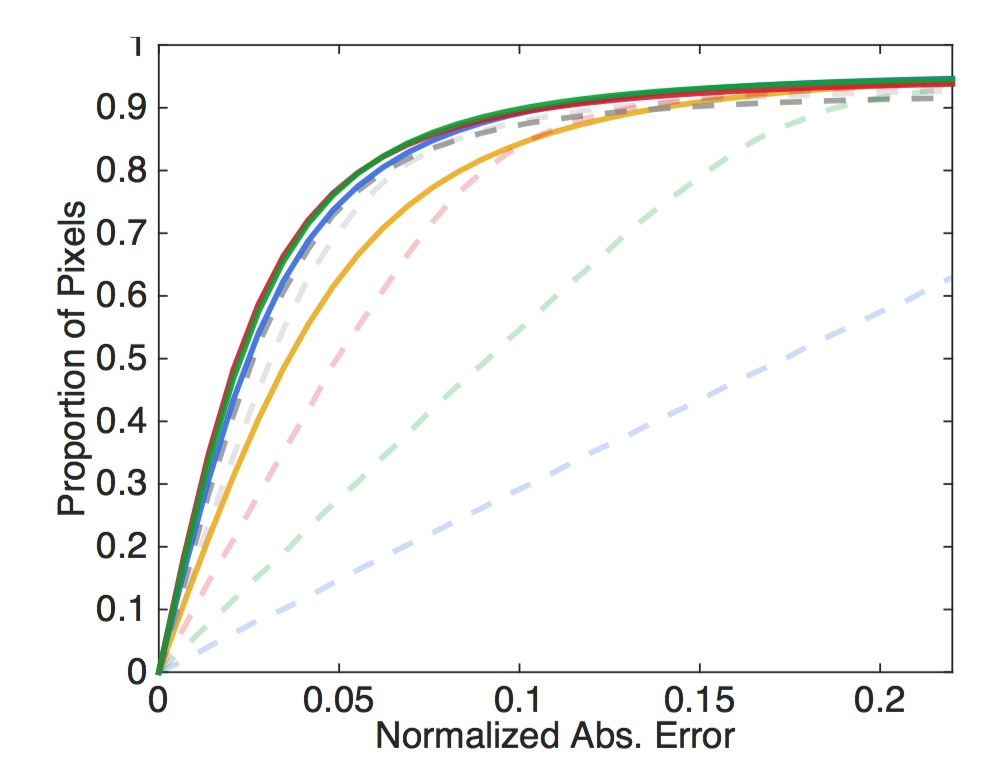
\includegraphics[trim={0.5cm 0.5cm 0.7cm 0.5cm},clip,width=0.9\textwidth]{Figures/Errorlar}
    \end{minipage}%
    \begin{minipage}{0.3\linewidth}
        \centering
        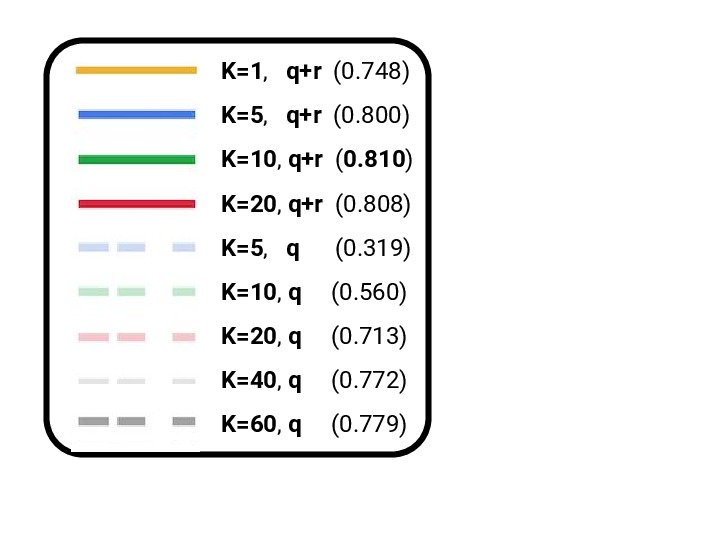
\includegraphics[trim={1.5cm 1cm 10cm 1cm},clip,width=1\textwidth]{Figures/Labels5-3}
    \end{minipage}
    \vspace{-0.35cm}
    \caption{Performance of $q$ and $r$, branches for various tesselation granularities of the human face, $K$. Areas under the curve(AUC) are reported.}
    \vspace{-0.15cm}
    \label{fig:exp}
    \vspace{-0.15cm}

\end{figure}

\subsection{Supervisory Signals for Faces and Bodies}
\label{sec: supervisory_signal}

Different objects have different degrees of articulation. Hence, we have used different supervisory UV maps for faces and bodies. In particular, we found that it is sufficient to use as supervisory signal for faces two channels one of the U and one for the V coordinate and following the simple tessellation strategy defined Fig. \ref{fig:DiscreteFaces}. The network takes as input the three RGB channels and outputs three channels (one for the U coordinates, one for the V coordinates and one for tessellated coordinates). The training data have been produced by fitting a 3DMM that could describe both the identity, as well as the expression of a human face in "in-the-wild" images (see experimental result section for more details). 

On the other hand because body is a highly articulated object, with each part having each own self-occlusion maps (i.e., a hand or a foot can be occluded with the rest of the body being visible), we created a UV map per part. In total we split the body in 25 parts, as visualized in in Fig. \ref{fig:IUV}, and we applied quantised regression for each of the UV maps of the 25 body regions (parts). Hence, for the human body the network takes as input the three RGB channels of the image and outputs 75 channels. That is, three channels for each of the 25 parts (one for the U coordinates of the part, one for the V coordinates of the part and one for tessellated coordinates). 

\begin{figure*}[h!]
\begin{center}
   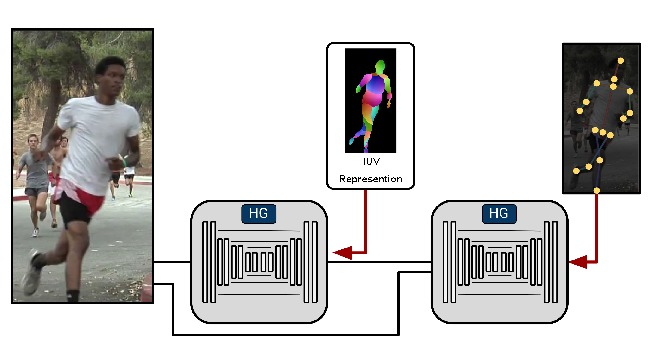
\includegraphics[width=0.49 \linewidth ]{Figures/PoseReg_Frontpage4-2}
   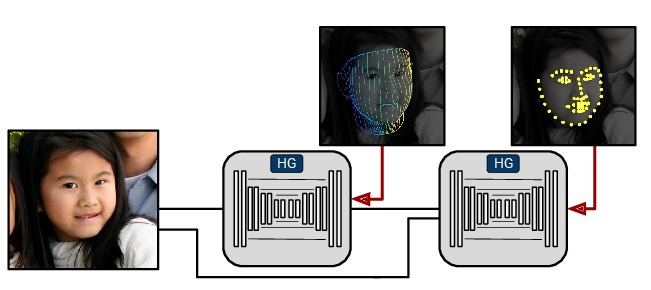
\includegraphics[width=0.49 \linewidth ]{Figures/PoseReg_Frontpage5-2}
\end{center}
   \caption{DenseReg cascade architecture for joint articulated pose estimation (body to the left, face to the right) and dense shape regression, wheredense correspondence supervision is obtained 3D Morphable Model fitting. Losses are shown in red. }
\label{fig:cascadeBody}
\end{figure*}

\subsection{A DenseReg Cascade for end-to-end dense shape regression and articulated pose estimation}
\label{sec: densereg_cascade}

Current algorithms for landmark localization and human pose estimation commonly address the learning problem in the form of a multi-class classification task, where each landmark defines its own class and the remainder of the image is labelled as background. Even though simple and effective, this training strategy provides a particularly sparse positive supervision signal, which asks a CNN to call everything other than a particular landmark a negative. We can intuitively say that our method simplifies this training `riddle', by providing information about dense correspondence between two surfaces. This fits  with the `Privileged Information' paradigm of  \citep{VapnikV09} where an `Intelligent Teacher' provides additional information during training that helps `understand' why a given  decision is taken. As a simple example, classifying a pixel as being a `knee' landmark can potentially be assisted by having dense correspondence maps, that  help the network solve the problem in a coarse-to-fine manner. Rather than rely on semantic supervision signals  we  rely on dense shape-level supervision.
 
Hence, motivated from the above we propose end-to-end trainable cascaded architectures which estimate dense correspondences and then these are used to improve articulated pose estimation. The architecture, coined DenseReg cascade, is depicted in Fig.~\ref{fig:cascadeBody}. In this particular, architecture the first network (which is in a form of hourglass) is used for dense shape regression. The output of the dense shape regression network is passed as privileged information in the second network which performs articulated body/face pose estimation. 


